% Figure: geometry of the organizing identity (1.4)/(2.8).
% Standalone TikZ source; compile with pdflatex. The same tikzpicture
% can be pasted into the manuscript (needs \usepackage{tikz} and the
% libraries below, plus amssymb/mathrsfs for the symbols).
\documentclass[border=2pt]{standalone}
\usepackage[T1]{fontenc}
\usepackage{lmodern}
\usepackage{amsmath,amssymb,mathrsfs}
\usepackage{tikz}
\usetikzlibrary{calc,arrows.meta}
\begin{document}
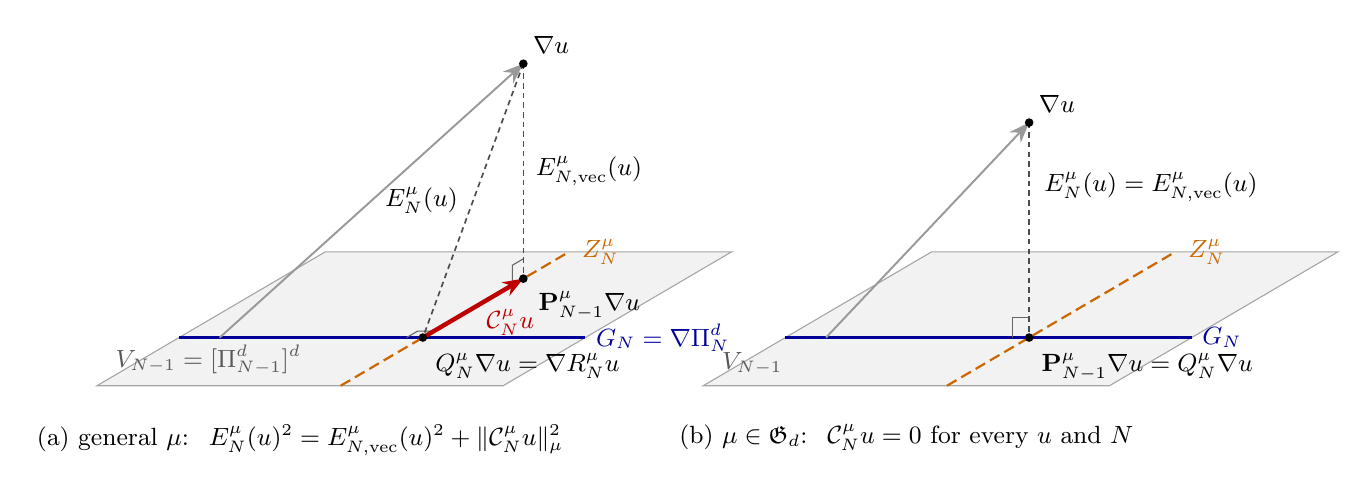
\begin{tikzpicture}[
  x={(0.86cm,0cm)}, y={(0.58cm,0.34cm)}, z={(0cm,1.05cm)},
  >={Stealth[length=2.6mm]},
  plane/.style={fill=black!5, draw=black!35, line width=0.4pt},
  gline/.style={draw=blue!60!black, line width=1.1pt},
  zline/.style={draw=orange!80!black, line width=0.8pt, dash pattern=on 4pt off 2pt},
  vec/.style={->, line width=0.9pt},
  defect/.style={->, draw=red!75!black, line width=1.6pt},
  leg/.style={line width=0.6pt, draw=black!70, dash pattern=on 2pt off 1.5pt},
  lab/.style={font=\small},
  dot/.style={circle, fill=black, inner sep=1.1pt},
]

% ------------------------------------------------------------------
% Panel (a): general measure
% ------------------------------------------------------------------
\begin{scope}
  % the plane V_{N-1}
  \filldraw[plane] (-0.6,-1.8,0) -- (5.4,-1.8,0) -- (5.4,3.2,0) -- (-0.6,3.2,0) -- cycle;
  \node[lab, anchor=south west, text=black!65] at (-0.5,-1.75,0)
       {$V_{N-1}=[\Pi^d_{N-1}]^d$};

  % G_N (line in the plane) and Z_N (its orthogonal complement in the plane)
  \draw[gline] (-0.6,0,0) -- (5.4,0,0)
       node[lab, anchor=west, text=blue!60!black] {$G_N=\nabla\Pi^d_N$};
  \draw[zline] (3,-1.8,0) -- (3,3.2,0)
       node[lab, anchor=west, text=orange!80!black, xshift=1pt]
       {$Z_N^\mu$};

  % points
  \coordinate (O)  at (0,0,0);
  \coordinate (Q)  at (3,0,0);      % Q_N^mu grad u = grad R_N^mu u
  \coordinate (P)  at (3,2.2,0);    % P_{N-1}^mu grad u
  \coordinate (G)  at (3,2.2,2.6);  % grad u

  % right-angle markers
  \def\ra{0.24}
  \draw[black!60, line width=0.4pt]
     ($(P)+(0,-\ra,0)$) -- ($(P)+(0,-\ra,\ra)$) -- ($(P)+(0,0,\ra)$);
  \draw[black!60, line width=0.4pt]
     ($(Q)+(-\ra,0,0)$) -- ($(Q)+(-\ra,\ra,0)$) -- ($(Q)+(0,\ra,0)$);

  % vectors from the origin
  \draw[vec, black!40, line width=0.7pt] (O) -- (G);

  % the right triangle
  \draw[leg] (G) -- (P);
  \draw[leg] (G) -- (Q);
  \draw[defect] (Q) -- (P);

  \node[dot] at (G) {};
  \node[dot] at (P) {};
  \node[dot] at (Q) {};

  % labels of points
  \node[lab, anchor=south west] at (G) {$\nabla u$};
  \node[lab, anchor=north west, xshift=2pt, yshift=-1pt] at (P) {$\mathbf P^\mu_{N-1}\nabla u$};
  \node[lab, anchor=north west, yshift=-2pt, xshift=1pt] at (Q)
       {$Q^\mu_N\nabla u=\nabla R^\mu_N u$};

  % lengths
  \node[lab, anchor=west, xshift=1pt] at ($(G)!0.5!(P)$) {$E^\mu_{N,\mathrm{vec}}(u)$};
  \node[lab, anchor=east, xshift=-2pt] at ($(G)!0.5!(Q)$) {$E^\mu_N(u)$};
  \node[lab, anchor=west, text=red!75!black, xshift=5pt, yshift=-3pt]
       at ($(Q)!0.4!(P)$) {$\mathcal C^\mu_N u$};

  % caption line for the panel
  \node[lab, anchor=north] at (2.4,-1.8,-0.35)
       {(a) general $\mu$: \ $E^\mu_N(u)^2=E^\mu_{N,\mathrm{vec}}(u)^2+\|\mathcal C^\mu_N u\|_\mu^2$};
\end{scope}

% ------------------------------------------------------------------
% Panel (b): compatible measure, mu in G_d
% ------------------------------------------------------------------
\begin{scope}[xshift=7.7cm]
  \filldraw[plane] (-0.6,-1.8,0) -- (5.4,-1.8,0) -- (5.4,3.2,0) -- (-0.6,3.2,0) -- cycle;
  \node[lab, anchor=south west, text=black!65] at (-0.5,-1.75,0)
       {$V_{N-1}$};

  \draw[gline] (-0.6,0,0) -- (5.4,0,0)
       node[lab, anchor=west, text=blue!60!black] {$G_N$};
  \draw[zline] (3,-1.8,0) -- (3,3.2,0)
       node[lab, anchor=west, text=orange!80!black, xshift=1pt] {$Z_N^\mu$};

  \coordinate (O)  at (0,0,0);
  \coordinate (Q)  at (3,0,0);
  \coordinate (G)  at (3,0,2.6);

  \def\ra{0.24}
  \draw[black!60, line width=0.4pt]
     ($(Q)+(-\ra,0,0)$) -- ($(Q)+(-\ra,0,\ra)$) -- ($(Q)+(0,0,\ra)$);

  \draw[vec, black!40, line width=0.7pt] (O) -- (G);
  \draw[leg] (G) -- (Q);
  \node[dot] at (G) {};
  \node[dot] at (Q) {};

  \node[lab, anchor=south west] at (G) {$\nabla u$};
  \node[lab, anchor=north west, yshift=-2pt, xshift=1pt] at (Q)
       {$\mathbf P^\mu_{N-1}\nabla u=Q^\mu_N\nabla u$};
  \node[lab, anchor=west, xshift=2pt] at ($(G)!0.3!(Q)$)
       {$E^\mu_N(u)=E^\mu_{N,\mathrm{vec}}(u)$};

  \node[lab, anchor=north] at (2.4,-1.8,-0.35)
       {(b) $\mu\in\mathfrak G_d$: \ $\mathcal C^\mu_N u=0$ for every $u$ and $N$};
\end{scope}
\end{tikzpicture}
\end{document}
